\section{DeepSmith}

DeepSmith\footnote{DeepSmith available at: https://chriscummins.cc/deepsmith} is our open source framework for compiler fuzzing. Figure~\ref{fig:deeptune} provides a high-level overview. The three key components of DeepSmith are: a generative model for random programs, a test harness, and voting heuristics for differential testing.

\begin{figure}[t!]
	\centering
	\begin{minipage}{.5\textwidth}
		\centering
		\vspace{-2em}
		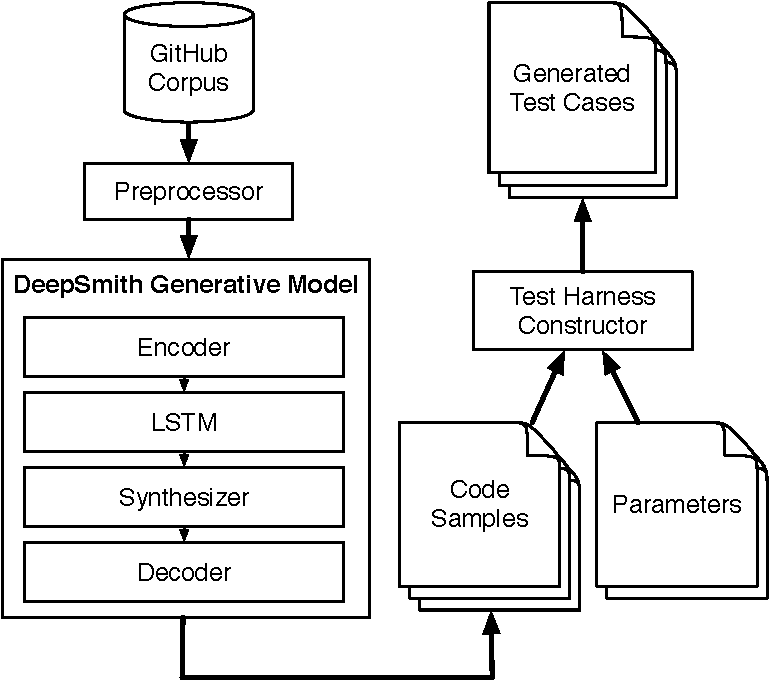
\includegraphics[width=.95\linewidth]{img/deepsmith}
		\captionof{figure}{DeepSmith system overview.}
		\vspace{-4em}
		\label{fig:deeptune}
	\end{minipage}%
	\begin{minipage}{.5\textwidth}
	\centering
	\vspace{-14em}
	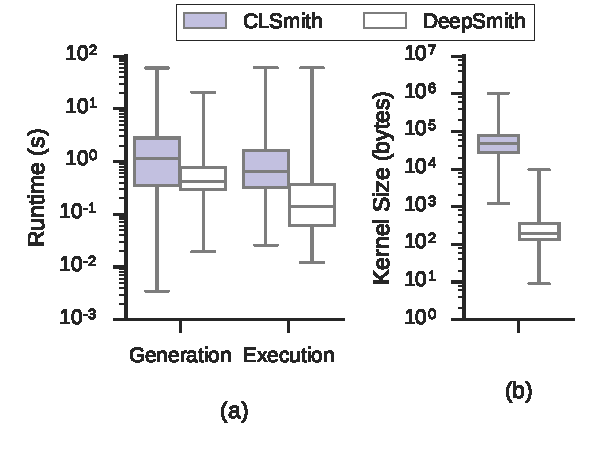
\includegraphics[width=\linewidth]{build/img/vs-clsmith}
	\vspace{-2.7em}
	\captionof{figure}{Comparison of runtimes (a) and test case sizes (b).}
	\label{fig:vs_clsmith}
\end{minipage}\\*
\begin{flushright}
\begin{minipage}{.5\textwidth}
	\centering
	\vspace{-12em}
	\includegraphics[width=\linewidth]{build/img/clang-crashes}
	\vspace{-2em}
	\captionof{figure}{Crash rate of the Clang front-end of every LLVM release in the past 24 months compiling 75k DeepSmith kernels.}
	\label{fig:clangs}
\end{minipage}%
\end{flushright}
\end{figure}

\paragraph{Generative Model} Generating test cases for compilers is hard because their inputs are highly structured. Producing text with the right structure requires expert knowledge and a significant engineering effort, which has to be repeated from scratch for each new language. Instead, we treat the problem as an unsupervised machine learning task, employing state-of-the-art deep learning techniques to build models for how humans write programs. Our approach is inspired by breakthrough results in modeling challenging and high dimensional datasets through unsupervised learning~\cite{Raghu2016}. Contrary to existing tools, our approach does not require expert knowledge of the target language and is only a few hundred lines of code. We automated the assembly of this corpus by mining 10k OpenCL kernels from open source repositories on GitHub. We used an \emph{oracle compiler} (LLVM 3.9) to statically check the source files, discarding files that are not well-formed. This corpus, exceeding one million lines of code, is used as a representative sample of OpenCL code from which a generative model can be derived.

% \paragraph{Encoder}
The textual representation of program codes must be encoded as numeric sequences for feeding as input to the machine learning model. Prior machine learning works have used character-level encodings, token-level encodings, or fixed length feature vectors. We extend the hybrid character/token-level encoding of~\cite{Cummins2017b}, in which a programming language's keywords and common names are treated as individual tokens while the rest of the text is encoded on a character-level basis. This approach hits a balance between compressing the input text and keeping the number of tokens in the vocabulary low.

We additionally employed semantic-preserving transformations to simplify the training programs. First, each source file is preprocessed to expand macros and remove conditional compilation and comments. Then, all user-declared identifiers are renamed using an arbitrary, but consistent pattern based on their order of declaration: $\{a,\allowbreak b,\allowbreak c,\allowbreak \ldots,\allowbreak aa,\allowbreak ab,\allowbreak ac,\allowbreak \ldots\}$ for variables and $\{A,\allowbreak B,\allowbreak C,\allowbreak \ldots,\allowbreak AA,\allowbreak AB,\allowbreak AC,\allowbreak \ldots\}$ for functions. This ensures a consistent naming convention, without modifying program behavior. Finally, a uniform code style is enforced to ensure consistent use of braces, parentheses, and white space. These rewriting simplifications give more opportunities for the model to learn the structure and deeper aspects of the language and speed up the learning. On the other hand, some bugs in the preprocessor or front-end might no longer be discoverable. We reason that this is an acceptable trade-off. For languages where the corpus can be many orders of magnitude larger, for example, C or Java, models may be generated without these modifications.

% \paragraph{Neural Network}
We use the Long Short-Term Memory (LSTM) architecture of Recurrent Neural Network to model program code~\cite{Hochreiter1997}. In the LSTM architecture activations are learned with respect not just to their current inputs but to previous inputs in a sequence. In our case, this allows modeling the probability of a token appearing in the text given a history of previously seen tokens. Our LSTM networks model the vocabulary distribution over the encoded corpus. We used a two layer LSTM network of 512 nodes each, trained using Stochastic Gradient Descent for 50 epochs, with an initial learning rate of 0.002 and decaying by a factor of a half every 5 epochs.

Training the model on the OpenCL corpus took 12 hours using a single NVIDIA Tesla P40. We provided the model with no prior knowledge of the structure or syntax of a programming language.

% \paragraph{Program Generation}
The trained network is sampled to generate new programs. The model is seeded with the start of a kernel (identified in OpenCL using the keywords \texttt{kernel void}), and sampled token-by-token. A ``bracket depth'' counter is incremented or decremented upon production of \texttt{\{} or \texttt{\}} tokens respectively, so that the end of the kernel can be detected and sampling halted. The generated sequence of tokens is then decoded back to text and used for compiler testing.


\paragraph{Test Harness} OpenCL is an embedded compute kernel language, requiring host code to compile, execute, and transfer data between the host and device. For the purpose of compiler fuzzing, this requires a \emph{test harness} to run the generated OpenCL programs. At first, we used the test harness of CLSmith. The harness assumes a kernel with no input and a \texttt{ulong} buffer as its single argument where the result is written. Only 0.2\% of the GitHub kernels share this structure. We desired a more flexible harness so as to test a more expressive range of programs, capable of supporting multi-argument kernels and generating data to use as inputs.

We developed a harness which first determines the expected arguments from the function prototype and generates host data for them. At the moment, we support scalars and arrays of all OpenCL primitive and vector types. For a kernel execution across $n$ threads, buffers of size $n$ are allocated for pointer arguments and populated with values {$[1 \ldots n]$}; scalar inputs are given value $n$, since we observe that most kernels use these for specifying buffer sizes.

The training programs from which the generative model is created are real programs, and as such do not share the argument type restrictions. The model, therefore, may generate correct programs for which our driver cannot create example inputs. In this case, a ``compile-only'' stub is used, which only compiles the kernel, without generating input data or executing the compiled kernel.

Unlike the generative model, this test harness is language-specific and the design stems from domain knowledge. Still, it is a relatively simple procedure, consisting of a few hundred lines of Python.

% \subsection{Voting Heuristics for Differential Testing}

We employ established Differential Testing methodologies to expose compiler defects. As in prior work, voting on the output of programs across compilers has been used to circumvent the \emph{oracle problem} and detect miscompilations~\cite{McKeeman1998}. However, we extend this approach to describe not only miscompilations, but also anomalous build failures and crashes.


%
%\begin{enumerate}
%	\item \emph{Build failure} (\abf) Online compilation of the OpenCL kernel fails, usually accompanied by an error diagnostic.
%	\item \emph{Build crash} (\bc) The compiler crashes during online compilation of the OpenCL kernel.
%	\item \emph{Build timeout} (\bto) Online compilation of the OpenCL kernel exceeds the timeout of 60 seconds.
%	\item \emph{Runtime crash} (\arc) Compilation of the OpenCL kernel succeeds gracefully, but the program crashes during kernel execution.
%	\item \emph{Runtime timeout} (\textbf{to}) Compilation of the OpenCL kernel succeeds gracefully, but program execution exceeds the timeout of 60 second.
%	\item \textbf{\cmark} \emph{Completion} The program terminates gracefully and produces an output.
%\end{enumerate}

When evaluating the outcomes of test cases, build crash (\bc) and build timeout (\bto) outcomes are of immediate interest, indicative of erroneous compiler behavior (examples may be found in Section~\ref{subsec:compile-time-defects}). For all other outcomes, \emph{differential tests} are required to confirm anomalous behavior. We look for test cases where there is a majority outcome -- i.e. for which some fraction of the testbeds behave the same -- but some testbed deviates. We use the presence of the majority increasing the likelihood that there is a `correct' behavior for the test case. In this work, we choose the majority fraction to be $\ceil{\frac{2}{3}n}$, where $n$ is the number of testbeds.
